\documentclass{beamer}
\usepackage[spanish]{babel}
\usepackage[latin1]{inputenc}
\usepackage{multicol} % indice en 2 columnas
\usepackage{graphics, graphicx}
\usepackage{listings}             % Incluye el paquete listings


\usetheme{Warsaw}
\usecolortheme{seahorse}
\useoutertheme{shadow}
\useinnertheme{rectangles}
\graphicspath{ {/home/emanuel/Tesis/Tesis/Documentos/img/} }

\setbeamertemplate{navigation symbols}{} % quitar simbolitos


\title[]{Optimizaci\'on del c\'omputo para la resoluci\'on del problema de una y dos part\'iculas en un pozo de potencial usando B-splines}
\author[]{Emanuel Lupi}

\institute[]
{
  Universidad Nacional de C\'ordoba\\
  FaMAF
}
\date{\today}

\begin{document}

\frame{\titlepage}

\section{Introducci\'on}
\subsection{Ecuaci\'on de Sch\"odringer}

\begin{frame}
  \frametitle{Introducci\'on}
  \begin{block}{Ecuaci\'on de Sch\"odringer}
    \begin{displaymath}
        E\psi(r) = \left[\frac{-\hbar^2}{2\mu} \nabla^2 + V(r)\right]\psi(r)
    \end{displaymath}
  \end{block}

  \begin{block}{Ecuaci\'on de Schr\"odinger independiente del tiempo}
      \begin{displaymath}\label{ec_schrodinger}
        \mathcal{H} |\psi_n(\vec{r})\rangle = E_n |\psi_n(\vec{r})\rangle\,,
      \end{displaymath}
  \end{block}

  \begin{block}{Ecuaci\'on radial}
    \begin{displaymath}
        -\frac{\hbar^2}{2m} \frac{1}{r^2}\frac{d}{dr}\left(r^2\frac{dR_n(r)}{dr}\right) 
        + \frac{\hbar^2\,l(l+1)}{2m\,r^2}\,R_n(r) + V(r)\,R_n(r) = E_n\,R_n(r)\,.
    \end{displaymath}
  \end{block}
\end{frame}


\begin{frame}
  \frametitle{Discretizaci\'on}
    
  \begin{displaymath}
    \phi_n(r) = r\,R_n(r)\,,
  \end{displaymath} 

  \begin{displaymath}
    -\frac{1}{2} \frac{d^2 \phi_n}{dr^2} + \frac{l(l+1)}{2\,r^2} \phi_n(r) + V(r)\,\phi_n(r) = E_n\,\phi_n(r)\,,
  \end{displaymath} 
  con las condiciones de contorno $\phi_n(r=0)=\phi_n(\infty) = 0$.
  \begin{displaymath}\label{combinacion_lineal}
      \phi_n(r) = \sum_{i=1}^{N} \alpha_i\,\varphi_i(r)\,,
  \end{displaymath}
\end{frame}

\begin{frame}
    \begin{displaymath}\label{ec_auval}
    H_l \vec{\alpha} = E\,S\,\vec{\alpha}\,,
    \end{displaymath}

    \noindent 
    para $E$ y $\lbrace\alpha_i\rbrace_1^N$, d\'onde

    \begin{align}\label{elemento_matriz}
    (H_l)_{ij} &= -\frac{1}{2} \int_0^{r_{max}} \varphi_i(r) \frac{d^2}{dr^2}\varphi_j(r) \,dr \nonumber
               + \frac{l(l+1)}{2}\int_0^{r_{max}} \frac{\varphi_i(r) \,\varphi_j(r)}{r^2} \,dr \\
               & + \int_0^{r_{max}} \varphi_i(r)\,V(r)\,\varphi_j(r)\, dr \\
    (S)_{ij} &= \int_0^{r_{max}} \varphi_i(r)\,\varphi_j(r)\,dr \label{solapamiento}
    \end{align}
\end{frame}

\begin{frame}
  \frametitle{Extendiendo a dos Part\'iculas}

  \begin{displaymath}\label{hamiltoniano2p}
    \mathcal{H}_{2p} = \mathcal{H}_{1p}^{(1)} + \mathcal{H}_{1p}^{(2)} + U(\vec{r}_1,\vec{r}_2)\,,
  \end{displaymath}
  \begin{displaymath}\label{eq:scho-2p}
    \mathcal{H}_{2p} \psi_n(\vec{r}_1,\vec{r}_2) = E_n^{2p} \psi_n(\vec{r}_1,\vec{r}_2)\,,
  \end{displaymath}
  \begin{displaymath}\label{base-2p}
    \chi_{i,j}(r_1,r_2) = \left\lbrace \begin{array}{ccc}
                        \varphi_i(r_1)\,\varphi_j(r_2) & \mbox{si} & i=j \\
                        \frac{\varphi_i(r_1)\,\varphi_j(r_2)+\varphi_i(r_2)\,\varphi_j(r_1)}{\sqrt{2}} & \mbox{si} & i\neq j
                        \end{array} \right.\,,
  \end{displaymath}
  \begin{displaymath}\label{base-2p-2}
    \hat{\chi}_{i,j}(r_1,r_2) = \varphi_i(r_1)\,\varphi_j(r_2)\,,
  \end{displaymath}
  \begin{displaymath}\label{mat-hamiltoniano-2p}
    \begin{split}
    H_{i,i';j,j'} &= \langle \hat{\chi}_{i,j} |\mathcal{H}_{2p}|\hat{\chi}_{i',j'}\rangle \\
                  &= (H_l)_{i,i'}\,S_{j,j'} + S_{i,i'}\,(H_l)_{j,j'} + U_{i,i';j,j'}\,,
    \end{split}
  \end{displaymath}

  \begin{displaymath}\label{matriz_interaccion}
    \begin{split}
      U_{i,i';j,j'} &= \langle \chi_{i,j} |U(r_1,r_2)|\chi_{i',j'}\rangle \\
                    &=  \int_0^{r_{max}} \left(\int_0^{r_{max}} \varphi_i(r_1)\, \varphi_j(r_2)\,
                    U(r_1,r_2)\, \varphi_{i'}(r_1)\, \varphi_{j'}(r_2)\, dr_2\right)\, dr_1\,.
    \end{split}
  \end{displaymath}
\end{frame}

\begin{frame}
  \frametitle{El proceso}
  \textit{El m\'etodo que se optimiz\'o tiene las siguientes partes}
  \begin{itemize}
    \item {Armar el sistema
      \begin{itemize}
        \item El c\'alculo de las abscisas y pesos de la Cuadratura de Gauss-Legendre.
        \item C\'alculo de las matrices $H$ y $E$
        \item C\'alculo de la matriz U de interacci\'un. (En el sistema de 2 part\'iculas solamente)
        \item C\'alculo del sistema de dos part\'iculas $H_{2p}$ y $E_2$. (En el sistema de 2 part\'iculas solamente)
      \end{itemize}}
    \item {Resolver el sistema
  \begin{itemize}
    \item Usar alg\'un resolvedor de autovalores y autovectores con $H$ y $E$.
  \end{itemize}
  }
  \end{itemize}
\end{frame}

\section{Optimizaci\'on}
\subsection{Reducci\'on de la candidad de C\'alculos y Memoria}

\begin{frame}
  \frametitle{Matrices dispersas}
  \begin{figure}[!tbp]
    \centering
    \begin{minipage}[b]{0.4\textwidth}
      \includegraphics[width=\textwidth]{hsim20.eps}
      \caption{H L=20.}
    \end{minipage}
    \hfill
    \begin{minipage}[b]{0.5\textwidth}
        \includegraphics[width=\textwidth]{hsim50.eps}
        \caption{H L=50.}
    \end{minipage}
  \end{figure}

\end{frame}

\begin{frame}
  \frametitle{Matrices dispersas}
  \begin{figure}[!tbp]
    \centering
    \begin{minipage}[b]{0.5\textwidth}
      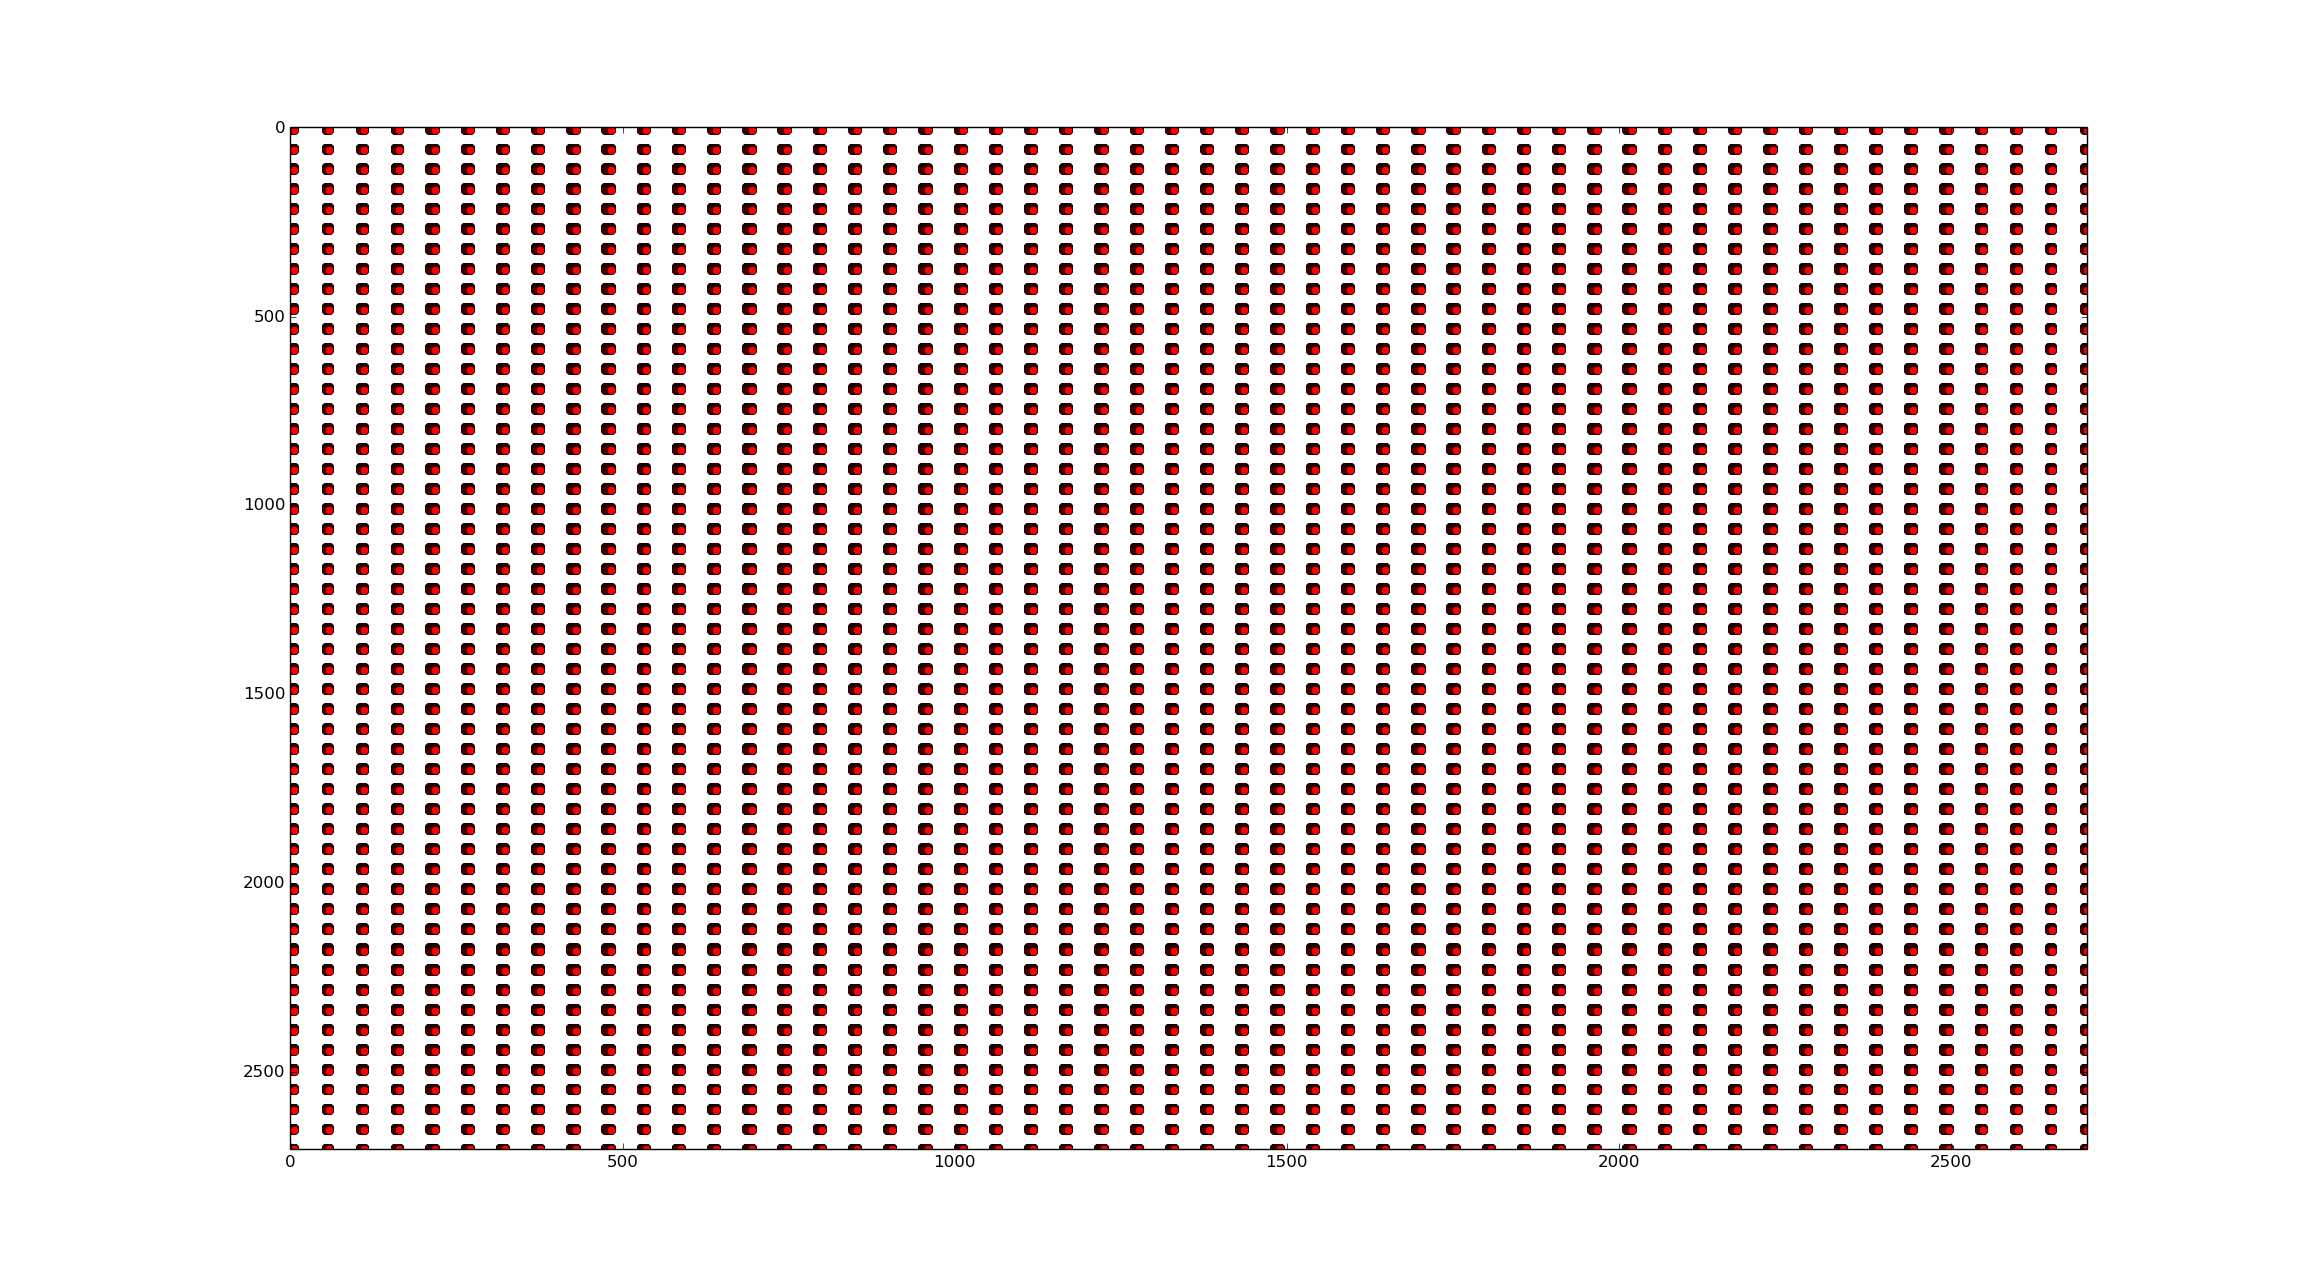
\includegraphics[width=\textwidth]{vef.eps}
      \caption{Matriz U.}
    \end{minipage}
    \hfill
    \begin{minipage}[b]{0.4\textwidth}
        \includegraphics[width=\textwidth]{matricita_vef.eps}
        \caption{Bloque de U.}
    \end{minipage}
  \end{figure}
\end{frame}

\begin{frame}
  \frametitle{Matrices dispersas}
  \begin{figure}[!tbp]
    \centering
    \includegraphics[width=0.7\linewidth]{smat.eps}
    \caption{Matriz S.}
  \end{figure}
\end{frame}

\lstset{language=C, breaklines=true, basicstyle=\footnotesize}


\defverbatim[colored]\lstI{
\begin{lstlisting}[
language=C++,
basicstyle=\ttfamily,
keywordstyle=\color{red},
basicstyle=\tiny,
tabsize=2,
showspaces=false]
for(unsigned int m = 1; m<KORD; ++m)
  for(unsigned int n = m; n<KORD; ++n)
    for(unsigned int j = 0; j<INT_G; ++j) {
      double bm = 0, bn = 0;
      rr = x[idx(k[i], j)];
      bm = bder(rr, m, KORD);
      bn = bder(rr, n, KORD);
      ...
    }
\end{lstlisting}
}

\defverbatim[colored]\lstII{
\begin{lstlisting}[
language=C++,
basicstyle=\ttfamily,
keywordstyle=\color{red},
basicstyle=\tiny,
tabsize=2,
showspaces=false]
for(unsigned int j = 0; j<INT_G; ++j) {
  rr = x[idx(k[i], j)];

  for(unsigned int m = 1; m<KORD; ++m) 
    bders[m] = bder(rr, m, KORD);

  for(unsigned int m = 1; m<KORD; ++m) 
    for(unsigned int n = m; n<KORD; ++n) {
      double  bm = bders[m],
              bn = bders[n];
      ...
    }
}
\end{lstlisting}
}

\begin{frame}{Refactorizaci\'on de C\'odigo}{}
  \textit{Antes}
  \lstI
  \textit{Despues}
  \lstII
\end{frame}

\begin{frame}{Rec\'alculo de funciones simples}{}
  \begin{displaymath}
    T(i) = \left\lbrace \begin{array}{ccc}
                        R_{min} & \mbox{si} & i < KORD \\
                        R_{min} + dr * i  & \mbox{si} & KORD \leq i < KORD + L_{INT}\\
                        R_{min} + dr *\\ (KORD + L_{INT} - 1) & \mbox{si} & KORD + L_{INT} \leq i
                        \end{array} \right.\,
  \end{displaymath}
\end{frame}


\end{document}